\section{Diagramme des projets}

Nous pr�sentons ici la gestion des projets.\\
\begin{itemize}
\item Projet : Repr�sente un objet contenant les donn�es d'un
projet. Apr�s sa cr�ation, il est stock� dans ProjetManager.\\
\item ProjetManager : C'est l'objet qui g�re les projets, il
s'occupe de leur cr�ation, recherche.\\
\item TeachingData : Il g�re le stockage des projets dans
leur int�gralit�. Le ProjetManager lui fait appel pour toutes les
op�rations.\\
\item Trash : C'est l'objet qui collecte tous les
projets mis � la poubelle par leur cr�ateurs. Il les conserve
jusqu'a leur suppression d�finitive.\\
\item TeachingManager : Il g�re l'ensemble des projets pour la cr�ation ou la suppression.\\
\end{itemize}
\begin{center}
\scalebox{0.6}{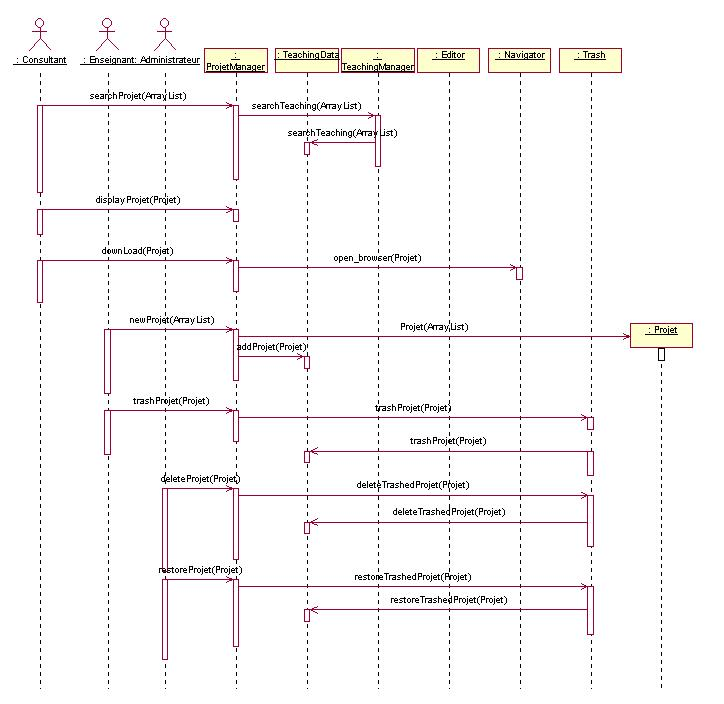
\includegraphics{images/projet.jpg}}\\
\par Diagramme de s�quence des projets\\
\end{center}


